\chapter*{Proposition 43}



\begin{figure*}[ht]
    \begin{center}
    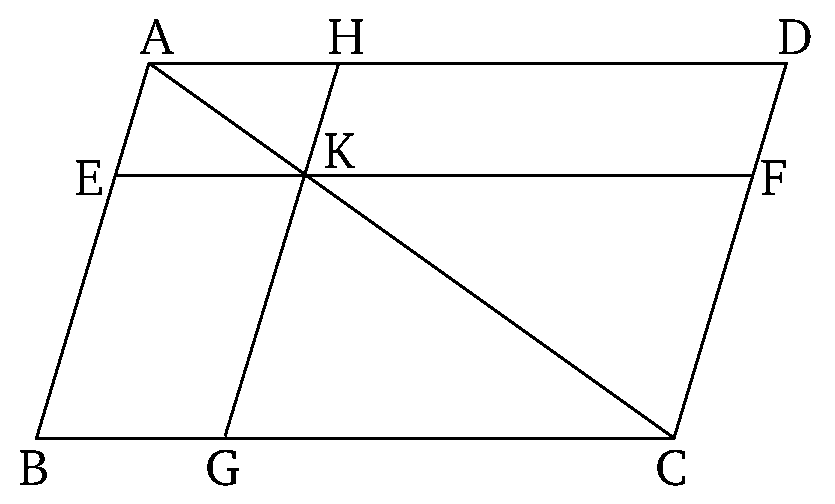
\includegraphics[width=0.5\linewidth]{figures/fig43e.eps}
    \label{fig:prop_43}
    \end{center}
\end{figure*}

For any parallelogram, the complements of the parallelograms about the diagonal are equal to one another.

Let $ABCD$ be a parallelogram, and $AC$ its diagonal. And let $EH$ and $FG$
be the parallelograms about  $AC$, and $BK$ and $KD$ the so-called complements
(about $AC$).
I say that the complement $BK$ is equal to the complement $KD$.

For since $ABCD$ is a parallelogram, and $AC$ its diagonal,  triangle
$ABC$ is equal to triangle $ACD$ [Prop.~1.34]. Again, since $EH$ is
a parallelogram, and $AK$ is its diagonal, triangle $AEK$ is equal to
triangle $AHK$ [Prop.~1.34]. So, for the same (reasons), triangle
$KFC$ is also equal to (triangle) $KGC$. Therefore, since triangle $AEK$ is
equal to triangle $AHK$, and $KFC$ to $KGC$, triangle $AEK$ plus $KGC$ is
equal to triangle $AHK$ plus $KFC$. And the whole triangle $ABC$ is
also equal to the whole (triangle) $ADC$. Thus, the remaining complement
$BK$ is equal to the remaining complement $KD$.

Thus, for any parallelogramic figure, the complements of the
parallelograms about the diagonal are equal to one another.
(Which is) the very thing it was required to show.


\section*{Commentary}

\begin{proposition}\label{proposition_43}\lean{Elements.Book1.proposition_43}\leanok
    If
\end{proposition}
\begin{proof}
    \uses{proposition_34}\leanok
\end{proof}
